%LTeX: language=it
\chapter{2020-03-20}
\section{Implicazioni Invarianza della Norma di un Quadrivettore}
Definiamo con \textbf{evento} l'insieme delle coordinate dello spazio a quattro
dimensioni, \textit{spazio di Minkowski}, che identificano un particolare
fenomeno fisico localizzato.
\begin{align}
	\textbf{Evento} \qquad \boxed{\qvec{P} = \mcb{ct,\vec{r}}}
\end{align}
Quindi supponiamo $\qvec{P}_1$ e $\qvec{P}_2$ due eventi dello spazio-tempo. La
distanza fra i due eventi sarà anch'essa un quadrivettore definito come segue:
\begin{equation}
	\qvec{\Delta S} = \mcb{c\Delta t, \Delta x, \Delta y, \Delta z}
\end{equation}
L'invariante di tale quadrivettore, con $K$ e $K^\prime$ due sistemi di
riferimento in moto relativo, poiché $\qvec{\Delta S}^2$ è invariante
relativistico:
\begin{align}
	K \longrightarrow \qvec{\Delta S}^2        & = \mrb{c \Delta t}^2 - \Delta x^2 -
	\Delta y^2 - \Delta z^2
	\\
	K^\prime \longrightarrow \qvec{\Delta S}^2 & = \mrb{c \Delta t^\prime}^2 -
	\Delta x^{\prime 2} - \Delta y^{\prime 2} - \Delta z^{\prime 2}
\end{align}

\paragraph{Classificazione del concetto di Distanza nello spazio di Minkowski}
Facendo riferimento agli eventi $\qvec{P}_1, \qvec{P}_2$, si definisce:
\begin{itemize}
	\item \textbf{distanza di tipo spazio (space-like)} $\rightarrow$ esiste un
	      sistema di riferimento in cui i due eventi sono \textbf{simultanei} solo
	      se:
	      \begin{equation}
		      \boxed{\qvec{\Delta S}^2 < 0}
	      \end{equation}
	      e si dice che l'intervallo $\qvec{\Delta S}$ è una distanza di tipo spazio
	      ($c \Delta t \mprime = 0$);
	\item \textbf{distanza di tipo tempo (time-like)} $\rightarrow$ esiste un
	      sistema di riferimento in cui i due eventi sono \textbf{contigui} solo se:
	      \begin{equation}
		      \boxed{\qvec{\Delta S}^2 > 0}
	      \end{equation}
	      e si dice che l'intervallo $\qvec{\Delta S}$ è una distanza di tipo tempo
	      ($\Delta x ^{\prime\, 2} + \Delta y ^{\prime\, 2} + \Delta z ^{\prime\, 2}
		      = 0$);
	\item \textbf{distanza di tipo luce} $\rightarrow$ la propagazione della luce
	      è descritta da:
	      \begin{equation}
		      \boxed{\qvec{\Delta S}^2 = 0}
	      \end{equation}
	      e si dice che l'intervallo $\qvec{\Delta S}$ è una distanza di tipo luce
	      ($c \Delta t ^{\prime\, 2} - \Delta x ^{\prime\, 2} - \Delta y ^{\prime\, 2}
		      - \Delta z ^{\prime\, 2} = 0$).
\end{itemize}

\begin{figure}[ht]
	\centering
	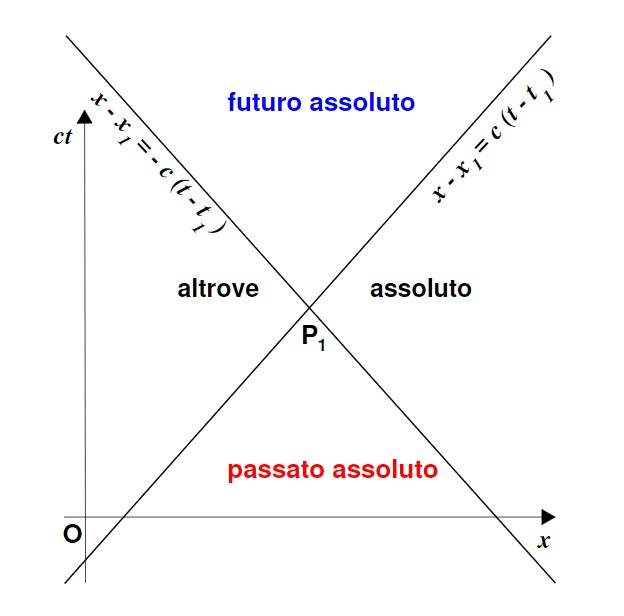
\includegraphics[scale=0.5]{./img/2020_03_20/minkowski.jpg}
	\caption{Spazio-Tempo di Minkowski unidimensionale relativo all'evento
		$\qvec{P}_1$ (origine)}
	\label{fig:minkowski}
\end{figure}

Le linee raffigurate rappresentano quelle che in una dimensione vengono
chiamate \textit{linee di luce} (in due dimensioni \textit{coni di luce}
ed in tre dimensioni \textit{iperconi di luce}). Le regioni dello spazio-tempo
interne alle linee di luce definiscono l'insieme degli eventi separati
dall'evento origine da distanze	di tipo tempo. Le regioni esterne alle linee di
luce, invece, definiscono l'insieme degli eventi separati dall'evento origine
da distanze di tipo spazio.

\section{Ulteriori Quadrivettori}
In aggiunta al quadrivettore posizione possiamo definire i seguenti
quadrivettori. Definiamo $t_0$ il \textbf{tempo proprio della particella},
ossia quello misurato nel sistema di riferimento che vede la particella in
quiete. Questo significa che\footnote{
	Tutte le variabili non apicate fanno riferimento al sistema di riferimento
	$K$ in moto relativo rispetto a $K^\prime$
}:
\begin{equation}
	\md{x}_0 = \md{y}_0 = \md{z}_0 = 0
	\mthen
	\md{s}^2 = c^2 \md{t}_0^2
\end{equation}
Dalla dilatazione temporale abbiamo:
\begin{equation}
	\md{t}_0 = \frac{\md{t}}{\gamma}
	\mthen
	\gamma = \mdv{t}{t_0}
\end{equation}
Quindi definiamo i seguenti quadrivettori:
\begin{itemize}
	\item \textbf{quadrivelocità}
	      \begin{equation}
		      \qvec{V} = \mdv{\qvec{X}}{t_0} = \mdv{\qvec{X}}{t} \mdv{t}{t_0} =
		      \gamma \mdv{\qvec{X}}{t}
		      \mthen
		      \boxed{
			      \qvec{V}
			      = \gamma\mdv{\qvec{X}}{t}
			      = \gamma \mcb{c,\vec{v}}
			      \equiv \mcb{\gamma c, \gamma \vec{v}}
		      }
	      \end{equation}
	      L'invariante della quadrivelocità:
	      \begin{equation}
		      \qvec{V}^2 = \gamma^2c^2 - \gamma^2\beta^2c^2 =
		      c^2\gamma^2\mrb{1-\beta^2} = c^2
	      \end{equation}

	\item \textbf{quadrimpulso}\footnote{
		      \textbf{Limite Classico}: per $\beta\to 0 \Rightarrow \gamma\to 1$ si
		      riottiene $\vec{p} = m\vec{v}$
	      }
	      \begin{equation}
		      \boxed{\qvec{P} = m \qvec{V} = m \gamma \mcb{c,\vec{v}}}
	      \end{equation}
	      con $m$ la \textit{massa a riposo} della particella.\par
	      L'invariante del quadrimpulso:
	      \begin{equation}
		      \qvec{P}^2 = m^2\gamma^2c^2 - m^2\gamma^2v^2 = m^2\gamma^2c^2 -
		      m^2\gamma^2\beta^2c^2 = m^2c^2\gamma^2\mrb{1-\beta^2} = m^2c^2
	      \end{equation}
\end{itemize}

\section{Energia}
\subsection{Energia a Riposo}
Definiamo l'energia a riposo di una particella come:
\begin{align}
	\textbf{Energia a riposo} \qquad \boxed{E_0 = m_0c^2}
\end{align}
dove $m_0$ è la massa a riposo della particella.

\subsection{Energia Relativistica}
Possiamo riscrivere il quadrimpulso come segue:
\begin{equation}
	\boxed{
		\qvec{P} = \mcb{\frac{E}{c}, \gamma\vec{p}}
	}
\end{equation}
dove $E$ è l'energia relativistica della particella e dove, per poter scrivere
la prima componente abbiamo sfruttato le seguenti identità:
\begin{equation}
	m_0 \gamma c = \frac{m_0 \gamma c^2}{c} = \frac{E_0\gamma}{c} = \frac{E}{c}
\end{equation}
\begin{align}
	\textbf{Energia Relativistica} \qquad \boxed{E = E_0\gamma = m_0 \gamma c^2}
\end{align}

\subsection{Energia Cinetica Relativistica}
Un altro modo per esprimere l'energia relativistica è come somma dell'energia a
riposo e dell'energia cinetica della particella, ovvero:
\begin{equation}
	E = E_0 + T
\end{equation}
Quindi segue che l'espressione esplicita dell'energia cinetica
relativistica\footnote{
	Attenzione: l'espressione dell'energia cinetica si può ricavare formalmente
	dal teorema delle forze vive utilizzando un'espressione relativisticamente
	corretta della forza (vedi Intro. Fisica Moderna)
}:
\begin{equation}
	\boxed{T = E - E_0 = m_0c^2\gamma - m_0c^2 = m_0c^2\mrb{\gamma - 1}}
\end{equation}

\subsubsection{Limite classico dell'energia cinetica}
Anche in questo caso, per riottenere l'espressione classica dell'energia
cinetica dobbiamo effettuare uno sviluppo al primo ordine del fattore $\gamma$
di Lorentz ($\gamma = 1 + \frac{1}{2}\beta^2$), quindi (ricordando la
definizione $\beta = \frac{v}{c}$):
\begin{equation}
	T_{\text{cl}} = mc^2\mrb{1+ \frac{1}{2}\beta^2 - 1} = \frac{1}{2}mc^2\beta^2 =
	\frac{1}{2}mv^2
\end{equation}

\section{Sistemi di due particelle}
Laddove possibile cercheremo di sfruttare gli invarianti relativistici
(\textit{invarianza della norma di un quadrivettore}), evitando il calcolo
delle trasformazioni di Lorentz per ottenere variabili cinematiche al passaggio
fra sistemi di riferimento.

Sfrutteremo in particolare:
\begin{itemize}
	\item utilizzo del \textit{principio di conservazione del quadrimpulso}:
	      \begin{equation}
		      \sum_{j=1}^{N_{\text{ini}}} P_j^{\text{ini}}
		      = \sum_{k=1}^{N_{\text{fin}}} P_k^{\text{fin}}
	      \end{equation}
	\item l'\textit{invariante relativistico associato} al quadrimpulso per
	      passare da un sistema di riferimento a un altro.
\end{itemize}
Negli esempi che seguono:
\begin{itemize}
	\item ricaveremo velocità e fattore di Lorentz,
	      $\gamma = \frac{1}{\sqrt{1 - \beta^2}}$, che ci portano dal \textit{sistema
		      di riferimento del laboratorio} al \textit{sistema di riferimento del
		      centro di massa} di due particelle;
	\item ricaveremo l'impulso e l'energia di una particella nel \textit{sistema
		      di riposo di un'altra};
	\item calcoleremo gli impulsi e le energie di due particelle \textit{nel
		      sistema del centro di massa} delle due particelle.
\end{itemize}

\begin{figure}[ht]
	\centering
	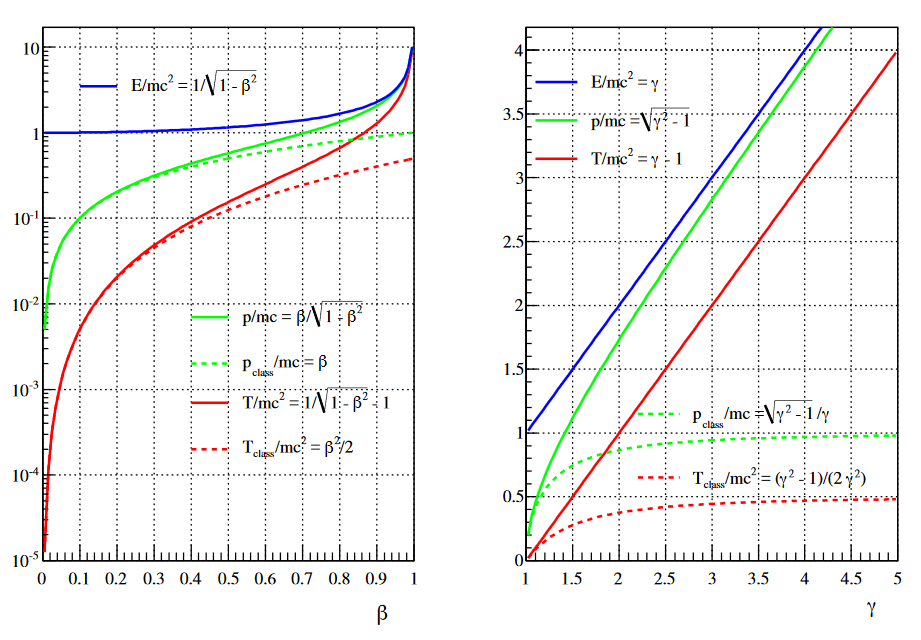
\includegraphics[scale=0.4]{./img/2020_03_20/realtivity_lectures.png}
	\caption{Energia totale, energia cinetica e impulso come funzioni di
		$\beta$ e $\gamma$ e rispettivi limiti classici ($\beta\to 0$)
	}
\end{figure}

\paragraph{Sistema di Unità Naturali}
D'ora in poi utilizzeremo il cosiddetto \textbf{sistema di unità naturali}, per
cui si fissano le costanti indicate di seguito pari all'unità:
\begin{equation}
	\boxed{\hbar = c = 1}
\end{equation}
e potremo scrivere \textit{uguaglianze fra grandezze fisiche non omogenee}
ricordandoci, però, di esprimere correttamente le unità di misura dei
risultati\footnote{
	Ad esempio, se un risultato di energia è $E = 1\si{\GeV}$, allora esprimeremo
	le grandezze $M,\vec{p}$ rispettivamente come $1\frac{\si{\GeV}}{c^2}$ e
	$1\frac{\si{\GeV}}{c}$
}.

Scriveremo il quadrimpulso come:
\begin{equation}
	\qvec{P} = \mcb{E,\vec{p}}
\end{equation}
e potremmo dire quindi:
\begin{equation}
	\qvec{P}^2 = E^2-\abs{\vec{p}\,}^2 = M^2
\end{equation}
\begin{equation}
	\textbf{Relazione di dispersione}
	\qquad
	\boxed{
		E^2 = \abs{\vec{p}\,}^2 + M^2
	}
\end{equation}
dove $M$ è detta \textbf{massa invariante} del sistema.

\subsection{Grandezze relative alla particella virtuale \quot{Centro di Massa}
	(CM)}
Le grandezze relative alle due particelle nel \textit{sistema del laboratorio}:
\begin{itemize}
	\item particella uno: $m_1,\ \qvec{P}_1$;
	\item particella due: $m_2,\ \qvec{P}_2$.
\end{itemize}
Nel sistema del laboratorio i due quadrimpulsi e i rispettivi invarianti
saranno:
\begin{equation}
	\qvec{P}_1 = \mcb{\varepsilon_1,\vec{p}_1}
	\mthen
	\qvec{P}_{1}^{2} = m_1^2
\end{equation}
\begin{equation}
	\qvec{P}_2 = \mcb{\varepsilon_2,\vec{p}_2}
	\mthen
	\qvec{P}_{2}^{2} = m_2^2
\end{equation}

\begin{note}[]
	D'ora in poi le quantità relative al sistema del centro di massa saranno
	espresse con un asterisco all'apice.
\end{note}

\begin{figure}[ht]
	\centering
	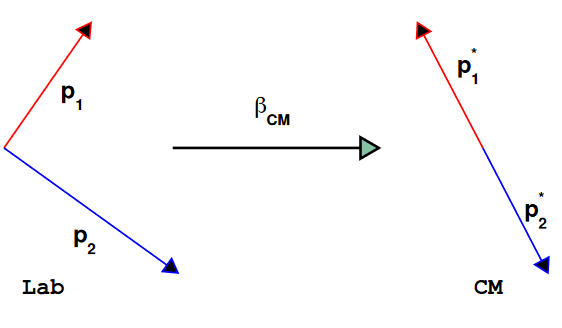
\includegraphics[scale=0.4]{./img/2020_03_20/particles1.png}
	\caption{Passaggio dal sistema del laboratorio al sistema del centro di massa
		\textbf{CM}}
	\label{fig:particles1}
\end{figure}

Il quadrivettore impulso totale, rispetto al \textit{sistema CM}:
\begin{equation}
	\qvec{P}^\ast
	= \qvec{P}_1^\ast + \qvec{P}_2^\ast
	= \mcb{\eps_1^\ast + \eps_2^\ast,\, 0}
\end{equation}
dato che nel sistema del centro di massa:
\begin{equation}
	\vec{p}_{1}^{\,\ast} + \vec{p}_{2}^{\,\ast} = 0
\end{equation}

Tramite una trasformazione di Lorentz del quadrimpulso si può riottenere
il quadrimpulso totale nel \textit{sistema del laboratorio}:
\begin{equation}
	\qvec{P}
	= \qvec{P}_1 + \qvec{P}_2
	= \mcb{\eps_1 + \eps_2,\, \vec{p}_1 + \vec{p}_2}
\end{equation}
Inoltre, per invarianza della norma, possiamo scrivere le seguenti
identità:
\begin{equation}
  \qvec{P}^2
	= E^{*2}
	= \mrb{\varepsilon_1^{\ast} + \varepsilon_2^{\ast}}^2
	= \mrb{\varepsilon_1 + \varepsilon_2}^2 - \mrb{\vec{p}_1 + \vec{p}_2}^2
\end{equation}
dove con $E ^{\ast}$ indichiamo l'\textbf{energia disponibile nel CM}.
Con $M$ la \textbf{massa invariante} totale del sistema, sfruttando
l'equazione precedente possiamo scrivere:
\begin{equation}
	\qvec{P}^2
	= \mrb{\qvec{P}_1 + \qvec{P}_2}^2
	= M^2
	= E^{\ast\,2}
	= \mrb{\varepsilon_1 + \varepsilon_2}^2 - \mrb{\vec{p}_1 + \vec{p}_2}^2
\end{equation}
Vediamo che massa invariante del sistema ed energia nel centro di massa
coincidono.

In questo modo abbiamo ridotto il problema di due particelle a un sistema di
\textbf{una sola particella virtuale \quot{centro di massa}} di quadrimpulso
$\qvec{P}$ ed massa $M = E^\ast$:
\begin{equation}
	\vec{p} = M\gamma\vec{\beta}_{\text{CM}}
\end{equation}
\begin{equation}
	E = M\gamma _{\text{CM}}
\end{equation}
dove $\vec{\beta}$ e $\gamma$ sono le velocità ed il fattore di Lorentz della
particella \textit{centro di massa} nel sistema del laboratorio:
\begin{equation}
	\boxed{\vec{\beta}_{\text{CM}}
	= \frac{\vec{p}}{E}
	= \frac{\vec{p}_1 + \vec{p}_2}{\varepsilon_1 + \varepsilon_2}}
	\label{eq:beta_CM}
\end{equation}
\begin{equation}
	\boxed{\gamma_{\text{CM}}
		= \frac{E}{M}
		= \frac{\varepsilon_1 + \varepsilon_2}{\sqrt{\mrb{\varepsilon_1 +
					\varepsilon_2}^2 - \mrb{\vec{p}_1 + \vec{p}_2}^2}}}
	\label{eq:gamma_CM}
\end{equation}

\subsection{Energia, impulso e velocità di una particella nel sistema di riposo
	dell'altra}
Nel sistema di riferimento $\textbf{RF}_1$, ovvero nel sistema di riferimento
solidale alla particella uno, i quadrivettori $\qvec{P}_1,\qvec{P}_2$:
\begin{equation}
	\qvec{P}_1 = \mcb{m_1,\, 0}
\end{equation}
\begin{equation}
	\qvec{P}_2 = \mcb{E_{2,1},\, \vec{p}_{2,1}}
\end{equation}

\begin{figure}[ht]
	\centering
	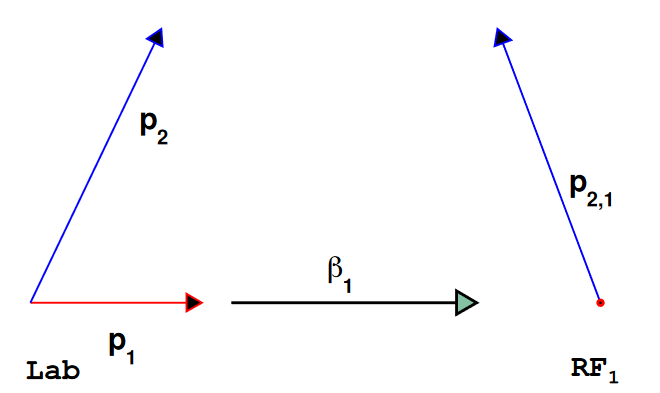
\includegraphics[scale=0.35]{./img/2020_03_20/relativity_lectures_1.png}
	\caption{Passaggio dal sistema del laboratorio al sistema di riferimento
		solidale alla particella uno, $\textbf{RF}_1$.}
\end{figure}

\begin{exercise}[]
	Dimostrare che il prodotto scalare fra quadrimpulsi è invariante
	relativistico.
\end{exercise}

\textit{Il prodotto scalare dei due quadrimpulsi è un invariante
	relativistico}, che vale:
\begin{equation}
	\qvec{P}_1 \qvec{P}_2 = m_1 E_{2,1}
	\mthen
	E_{2,1} = \frac{\qvec{P}_1 \qvec{P}_2}{m_1}
\end{equation}
inoltre, poiché possiamo scrivere:
\begin{equation}
	\abs{\vec{p}_{2,1}}^2 = E^2_{2,1} - m_2^2
\end{equation}
sostituendo l'espressione di $E _{2,1}$:
\begin{equation}
  \abs{\vec{p}_{2,1}}^2 = \frac{\qvec{P}_{1} \qvec{P}_{2}}{m_1} - m_2^2
\end{equation}
Per $\vec{\beta}_{2,1}$ possiamo scrivere:
\begin{equation}
  \abs{\vec{\beta}_{2,1}}^{2} = \frac{\abs{\vec{p}_{2,1}}^{2}}{E _{2,1}^{2}}
\end{equation}

Allora esprimiamo l'\textbf{energia}, l'\textbf{impulso} e la \textbf{velocità}
di una particella nel sistema di riposo dell'altra come, ovvero le grandezze
relative alla particella 2 nel sistema in cui la particella uno si trova in
quiete:
\begin{equation}
	\boxed{
		\begin{dcases}
			E_{2,1} = \frac{\qvec{P}_1\qvec{P}_2}{m_1}
			\\
			\abs{\vec{p}_{2,1}}^2
			= \frac{\mrb{\qvec{P}_{1} \qvec{P}_{2}}^{2}}{m_1^2} - m_2^2
			= \frac{\mrb{\qvec{P}_1\qvec{P}_2}^2 - m_1^2m_2^2}{m_1^2}
			\\
			\abs{\vec{\beta}_{2,1}}^2
			= \frac{\abs{\vec{p} _{2,1}}^{2}}{E _{2,1}^{2}}
			= \frac{\mrb{\qvec{P}_1\qvec{P}_2}^2 - m_1^2m_2^2}{\cancel{m_1^2}}
			\frac{\cancel{m_1^2}}{\mrb{\qvec{P}_{1} \qvec{P}_{2}}^{2}}
			= \frac{\mrb{\qvec{P}_1\qvec{P}_2}^2 -
				m_1^2m_2^2}{\mrb{\qvec{P}_1\qvec{P}_2}^2}
		\end{dcases}
	}
	\label{eq:sistema_riposo_altra}
\end{equation}
$\vec{\beta}_{2,1}$ rappresenta la \textit{velocità della particella due nel
	sistema di riferimento che vede la particella uno in quiete}.

